%!TEX root = ../main.tex
\clearpage
\section{Performance}
This section describes the performance of the controllers created in section~\ref{sec:controller}.
The controllers will be applied to both the real and the simulated system in order to compare the results.

\subsection{PI Controller}
The block diagram of this controller can be seen in figure~\ref{fig:pidcontroller}, although $K_D$ is set to zero in the PI controller.
Two tests are conducted for the PI controller, a load step and a velocity step.

\begin{figure}[!h]
	\centering
	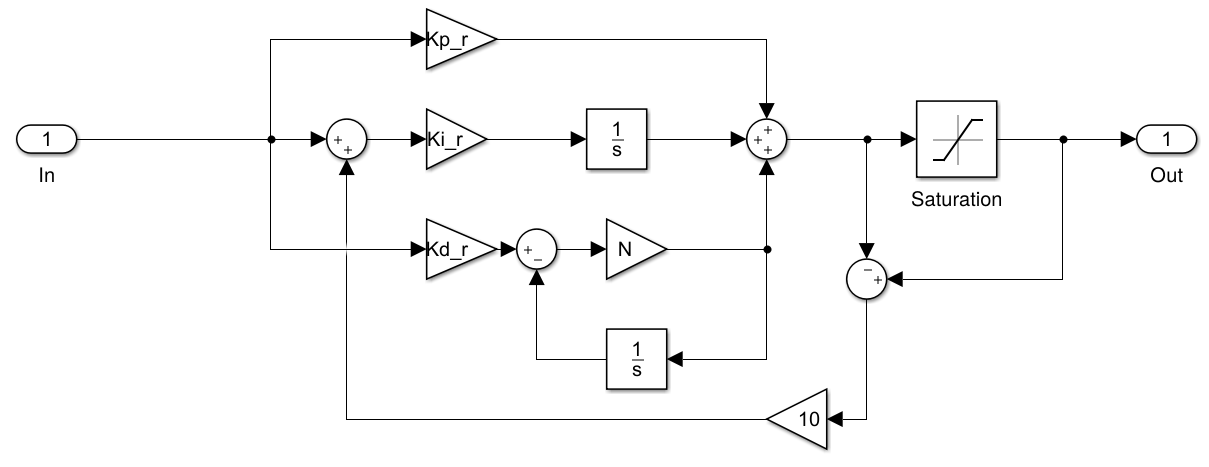
\includegraphics[width=.75\linewidth]{graphics/pid_controller}
	\caption{The implementation of the PID controller used with the dSpace system.}
	\label{fig:pidcontroller}
\end{figure}

\paragraph{Velocity Step:}~\\
A velocity step response was applied to the controller of values $\omega =$ 200, 250 and 400 $\frac{Rad}{S}$.
Note that at $\omega=400$ the controller was saturated significantly throughout the rise-time of the signal.
The result of these test can be seen on figure~\ref{fig:step}.
As it is expected when introducing an integral part to a controller, there is no appreciable steady-state error in either of the three cases.
There is, however, a ripple present on every test, most notably being at $\omega = 400$.
This is likely due to mechanical imperfections in the motor assembly.
Comparing the responses of the real and the simulated system in figures~\ref{fig:step200} and~\ref{fig:step200simulated}, respectively, although the real system has some overshoot that is not present in the simulation, the settling time is similar at $\approx50$ ms.

\begin{figure}[!h]
	\begin{subfigure}[t]{.49\linewidth}
		\centering
		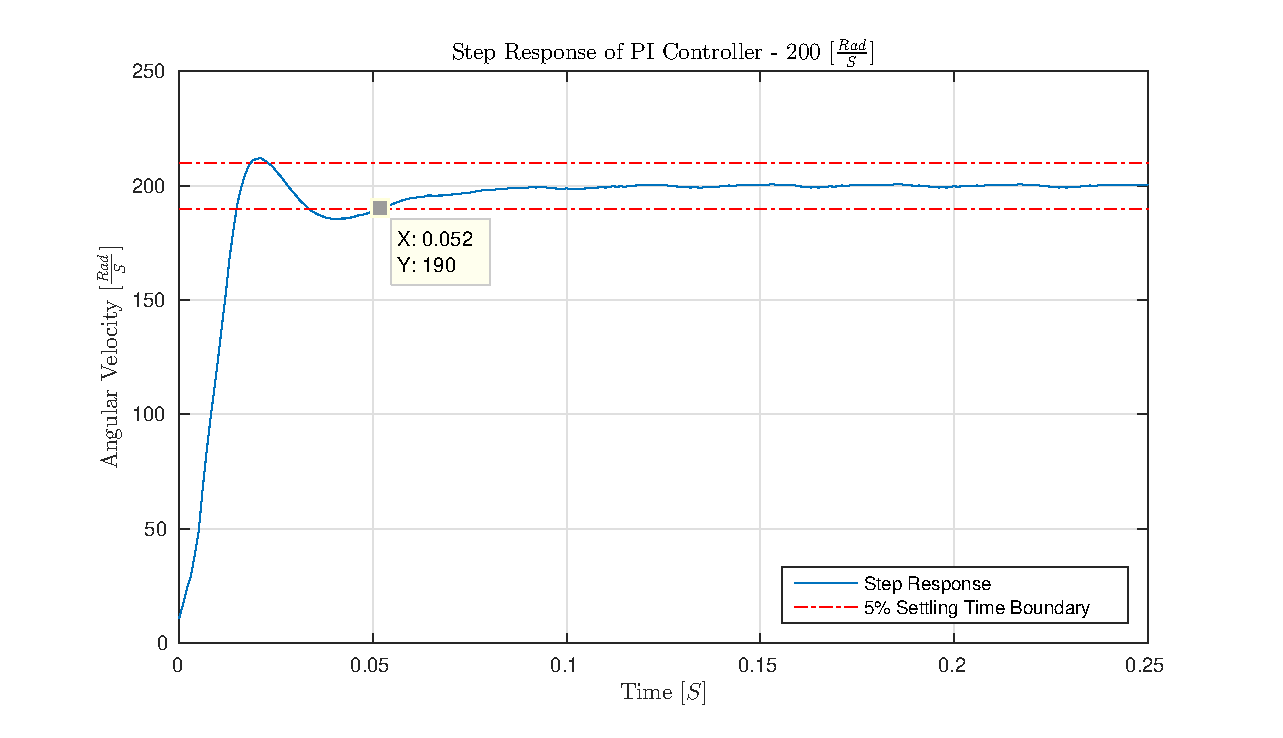
\includegraphics[width=\textwidth]{graphics/step_200_pi_real}
		\caption{Reference Step: $200 \frac{Rad}{S}$.}
		\label{fig:step200}
	\end{subfigure}
	\begin{subfigure}[t]{.49\linewidth}
		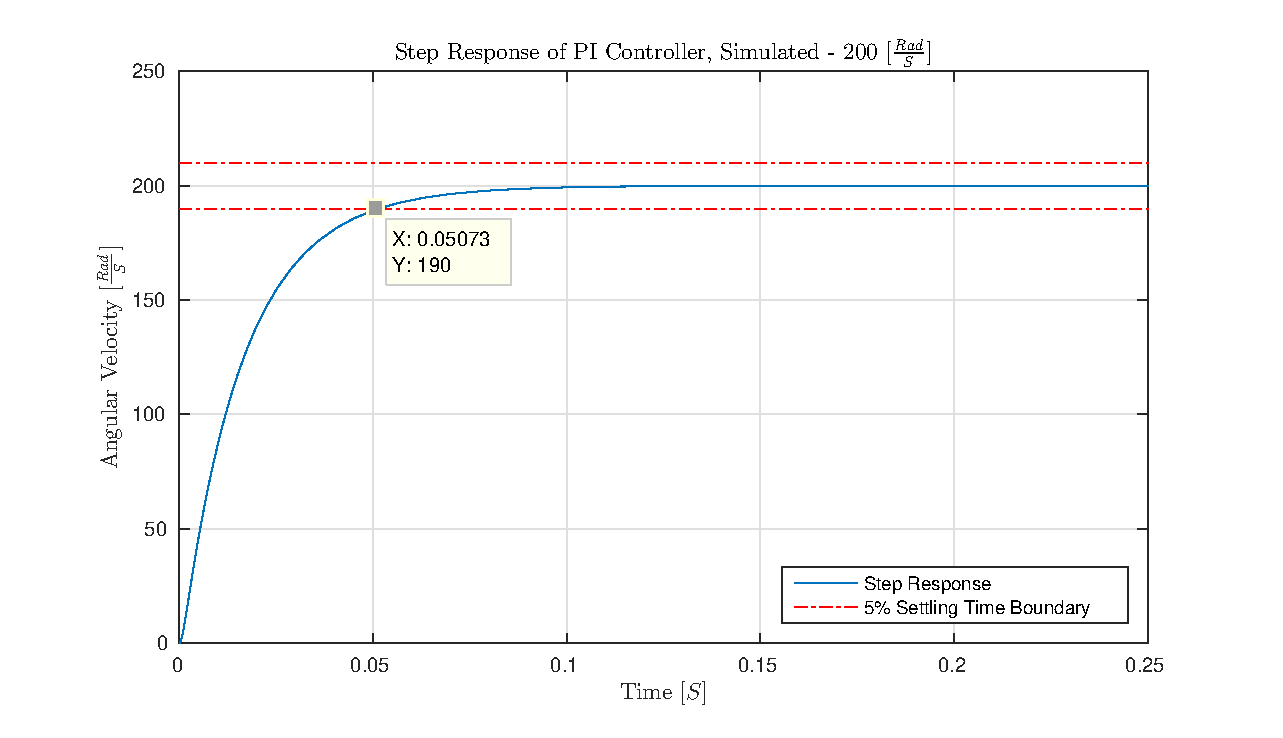
\includegraphics[width=\textwidth]{graphics/step_200_pi_simulated}
		\caption{Reference Step: $200 \frac{Rad}{S}$.}
		\label{fig:step200simulated}
	\end{subfigure}\\
	\centering
	\begin{subfigure}[t]{.49\linewidth}
		\centering
		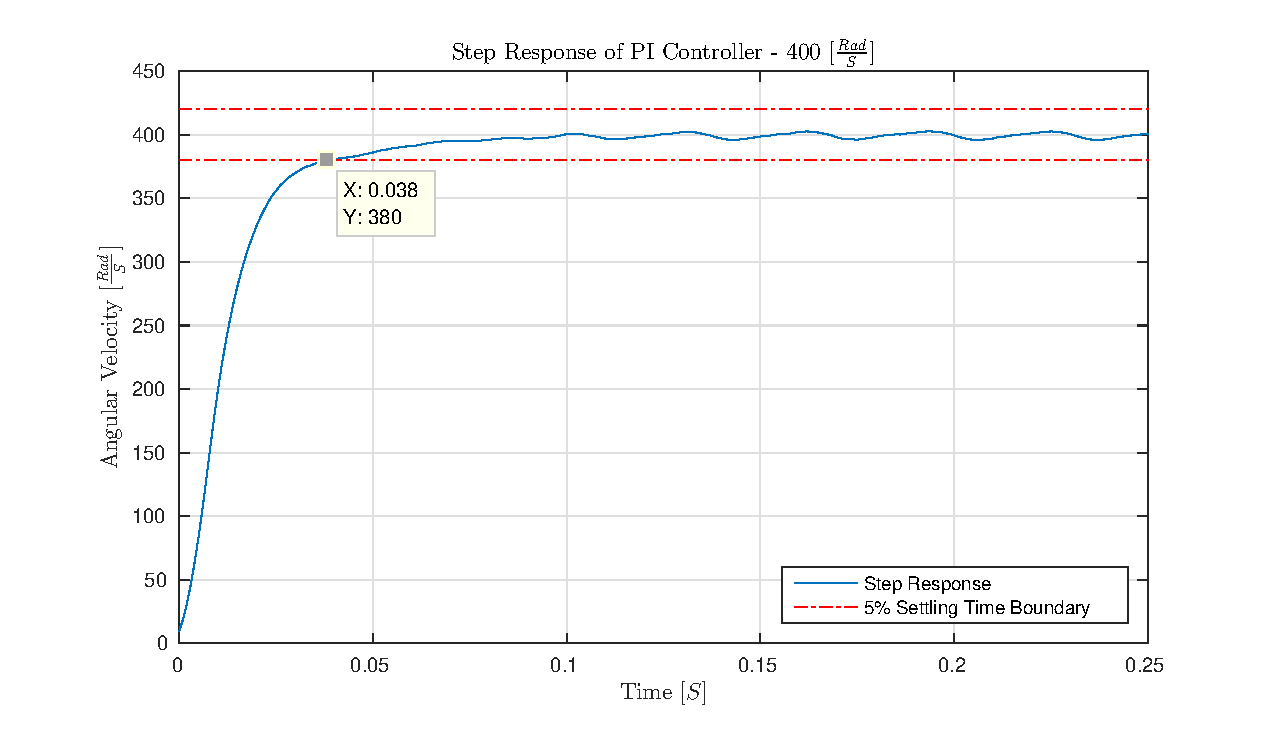
\includegraphics[width=\textwidth]{graphics/step_400_pi}
		\caption{Reference Step: $400 \frac{Rad}{S}$.}
		\label{fig:step400}
	\end{subfigure}
	\caption[Velocity step response of PI controller.]{Velocity step response of the PI controller. On each plot is marked the settling time of the response, $X$ in $[S]$.}
	\label{fig:step}
\end{figure}

Finally, the inertia was connected to the rotor of the motor and a reference step of $125\frac{Rad}{S}$ was applied.
As can be seen from~\ref{fig:stepinertia}, adding the extra inertia to the system greatly influences the performance of the controller.
The overshoot is greatly increased and the settling time lengthened by a factor of ten.
This is to be expected since the controller was designed without taking this inertia into account.
The responses in figures~\ref{fig:stepinertiareal} and~\ref{fig:stepinertiasimulated} are similar, but the overshoot on the real system is significantly higher than that on the simulated system.
This is likely due to the extra friction caused by bearings and other mechanical imperfections that are not modelled in the simulation.

\begin{figure}[!h]
	\begin{subfigure}[t]{.49\linewidth}
		\centering
		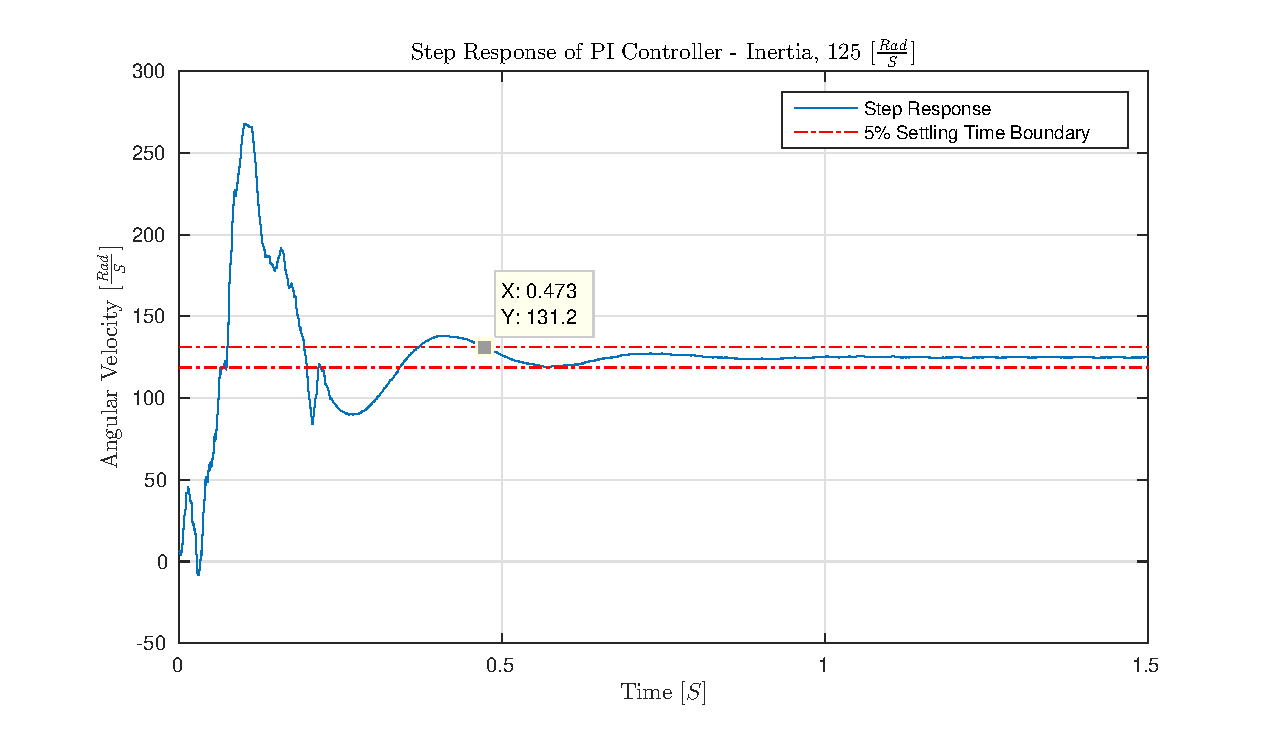
\includegraphics[width=\textwidth]{graphics/step_125_pi_inertia_real}
		\caption{Reference Step: $125 \frac{Rad}{S}$. Added inertia.}
		\label{fig:stepinertiareal}
	\end{subfigure}
	\begin{subfigure}[t]{.49\linewidth}
		\centering
		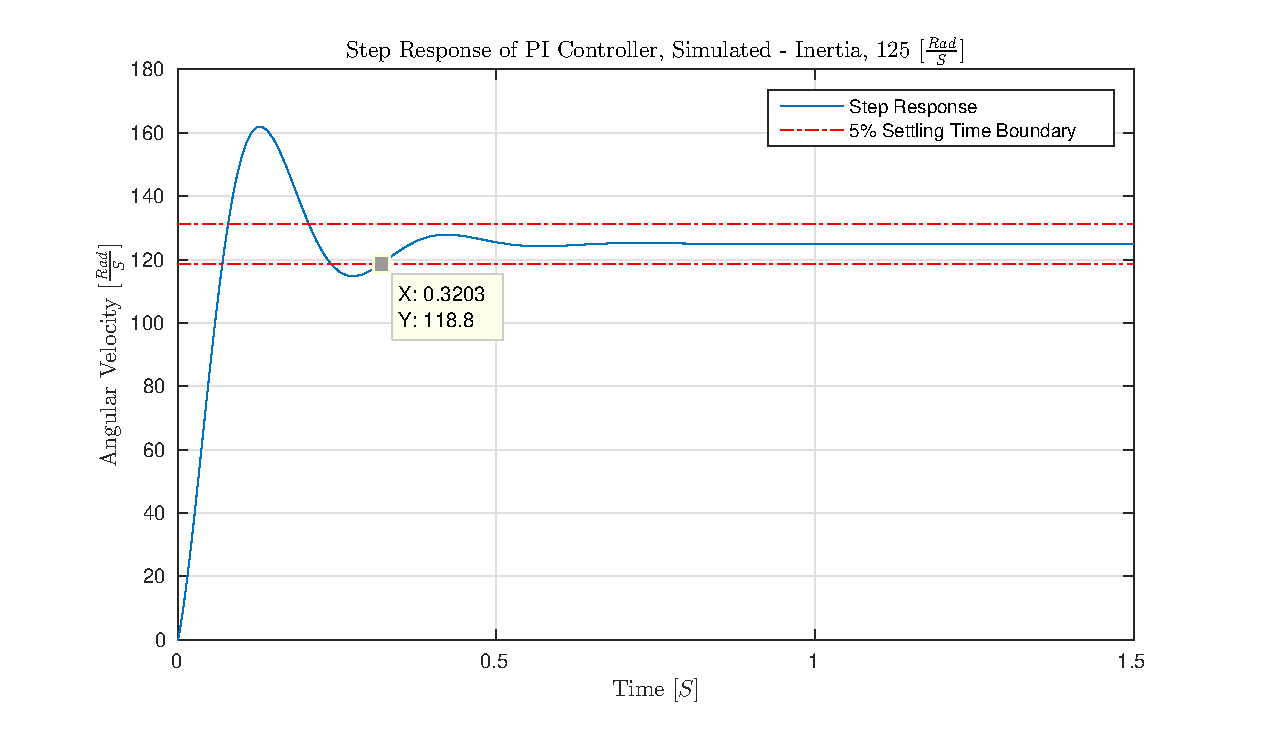
\includegraphics[width=\textwidth]{graphics/step_125_pi_inertia_simulated}
		\caption{Reference Step: $125 \frac{Rad}{S}$. Added inertia.}
		\label{fig:stepinertiasimulated}
	\end{subfigure}
	\caption[Velocity step response of PI controller with inertia.]{Velocity step response of the PI controller. On each plot the settling time of the response is marked, $X$ in $[S]$.}
	\label{fig:stepinertia}
\end{figure}

\paragraph{Load Step:}
The load step is performed by connecting both the inertia and the secondary motor to the rotor.
An electronic load is put in series with the terminals of the secondary motor.
This will allow for an easy way of limiting the current through the secondary motor, thus limiting the load generated.
The motor is now run at an angular velocity of $\omega=125\frac{Rad}{S}$.
Two loads were attempted: 0.4 and 0.5 $[A]$.
The results of this test can be seen in figure~\ref{fig:loadstep}.

\begin{figure}
	\begin{subfigure}[t]{.49\linewidth}
		\centering
		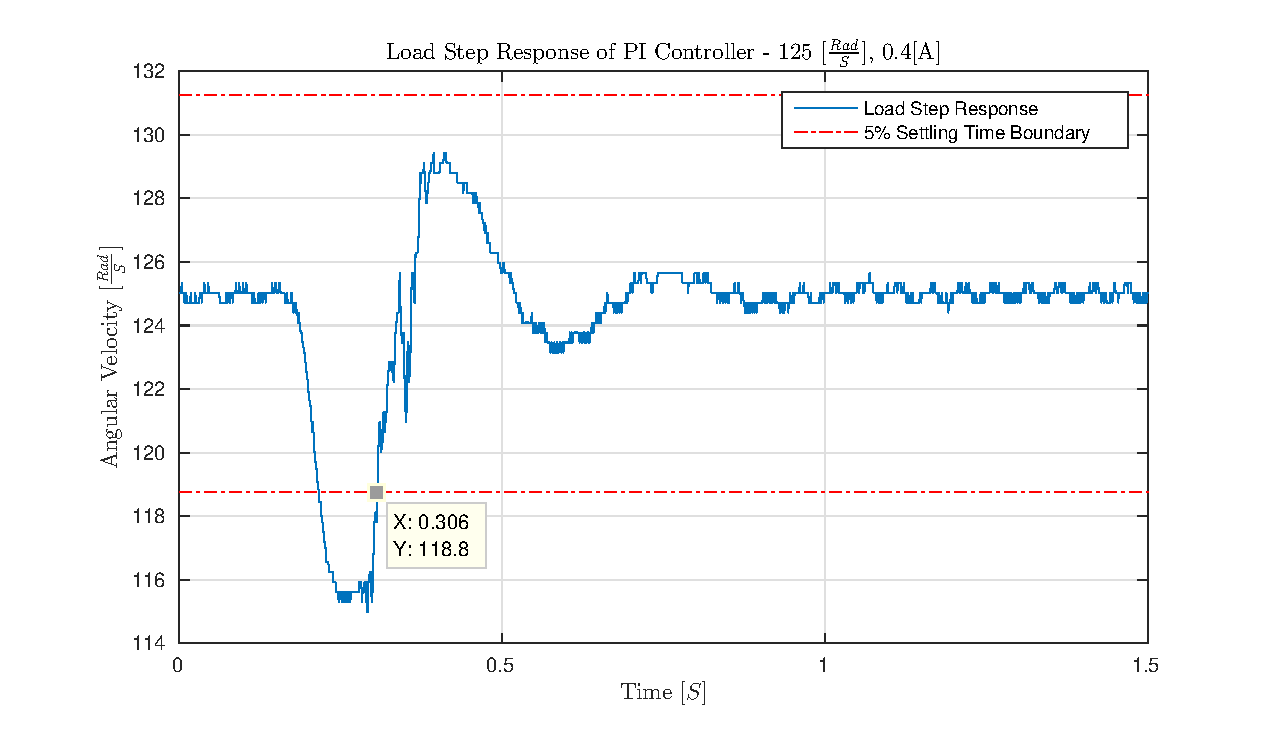
\includegraphics[width=\textwidth]{graphics/load_real}
		\caption{Reference Step: $0.4 [A]$.}
		\label{fig:loadstep04real}
	\end{subfigure}
	\begin{subfigure}[t]{.49\linewidth}
		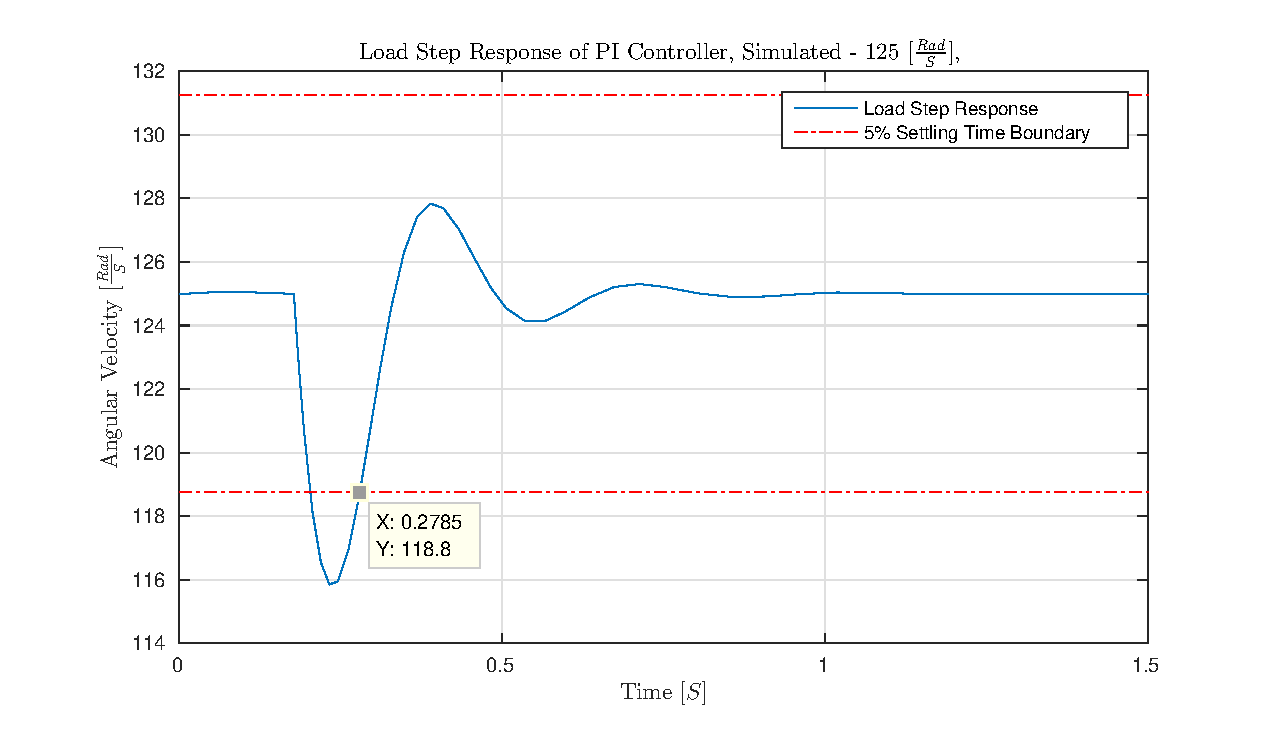
\includegraphics[width=\textwidth]{graphics/load_simulated}
		\caption{Reference Step: $0.4 [A]$.}
		\label{fig:loadstep04simulated}
	\end{subfigure}\\
	\centering
	\begin{subfigure}[t]{.49\linewidth}
		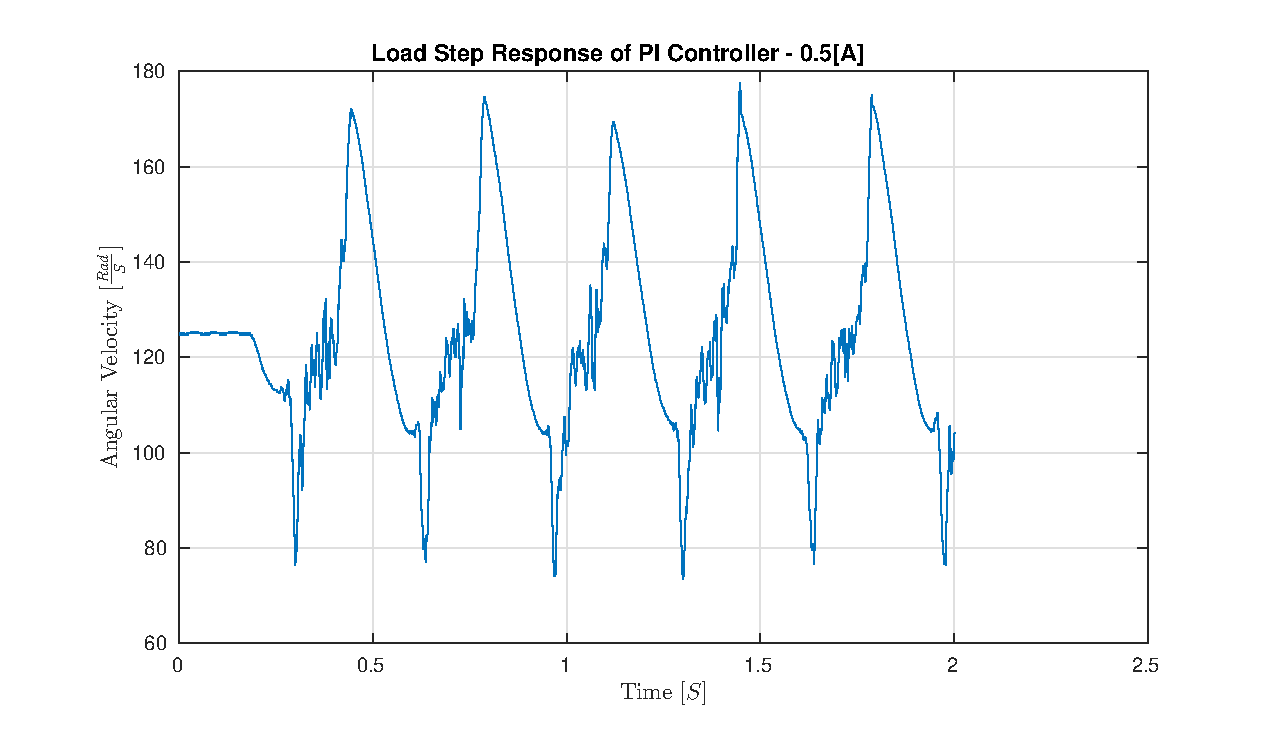
\includegraphics[width=\textwidth]{graphics/load_unstable}
		\caption{Reference Step: $0.5 [A]$.}
		\label{fig:}
	\end{subfigure}
	\caption[Load step response of PI controller]{Load step response of the PI controller. On each plot the settling time of the response is marked, $X$ in $[S]$.}
	\label{fig:loadstep}
\end{figure}

As can be seen, at the 0.5 $[A]$ reference step the controller becomes unstable.
The velocity continues to oscillate indefinitely.
Lowering the reference step slightly stabilises the response.
However due to the increased inertia on the system in this test the settling time is significant.
In this case, the real and simulated systems behaviours are very similar, both in settling time and the maximum and minimum peak values.
These can be seen in figures~\ref{fig:loadstep04real} and \ref{fig:loadstep04simulated} respectively.

\subsection{IPD Controller}
\begin{figure}[!h]
	\centering
	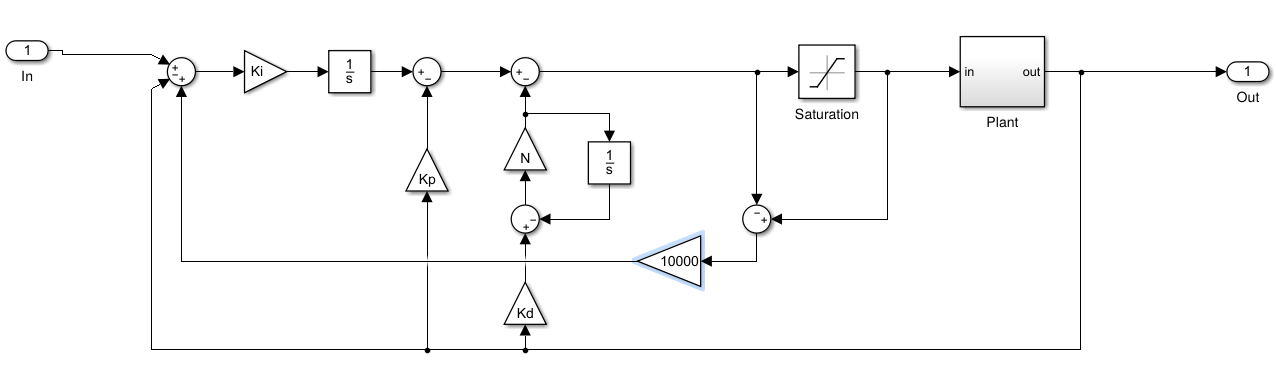
\includegraphics[width=.75\linewidth]{graphics/ipd_controller}
	\caption{The implementation of the IPD controller used with the dSpace system.}
	\label{fig:ipdcontroller}
\end{figure}

A Simulink block diagram of this controller can be seen in figure~\ref{fig:ipdcontroller}.
One difference between this controller and the PI controller described previously, is the inclusion of the differential gain. 
This inclusion gave rise to significant problems.
In order to have dSpace accepting the differential it was necessary to implement it as a low-pass filter.
By setting the cut-off frequency to a high value this filtering should have no effect on the system.
This was found to not be the case. 
At values above $\approx$1000$Hz$ the controller becomes unstable.
At these low values the filter still has a significant impact on the performance of the controller and it was not possible to obtain any sensible data on the performance of this controller.